\chapter{Problem Description}
\label{chp:relwork}
The nature of P2P systems is to help each other achieving a common purpose. In file-sharing P2P systems, the purpose is to obtain some particular content on the Internet. However, in reality, some peers are able to freeride. Although limited, an incentive system can push anyone to contribute. The distant future vision of this work is to create an \textit{European Youtube}-type of system without any central authority server. Similar to Youtube's ease-of-use, our system uses \bt~for robust seeding and without explicit file management or complicated settings. One of the benefits of this research is the existence of an automatic caching layer, which ensures content availability for both long-lived years-old and freshly-created content. It is desirable to deliver the autonomous mechanism where everyone contributes, and at the same time can gain benefit for themselves. Specifically, by devising a credit mining system, we take an important step to reduce the needs for human intervention in contributing to improve other users' experience.

In this chapter, the problems that are the main concern of this thesis will be elaborated. We will discuss performance problems in \bt~system, specifically by looking at its supply and demand misalignment. After that, the \textit{investment} as possible behavior that can tackle this issue will be elaborated. It covers the importance, potential gains, and desired effect of the possible credit investment. After specifying problems, prior works on credit mining will be reviewed. Further improvements on those works are the core of this thesis. Lastly, two research questions on investing in credit system will be formulated.
 

%\section{Cooperation and performance in \bt}
% the necessity to add more reputation management using cooperation. To monetize cooperation.
%Peer-to-peer file sharing community, especially \bt~ can improve the user downloading experience. It does not give strain to server connection and naturally will download as fast as possible depending on file availability. However, uncooperative peer behavior and low file availability can affect a swarm's health thus reducing download experience. 
%Several kinds of researches already provide solutions to prevent uncooperative peer behavior, all to indirectly push higher downloading throughput on downloader.
%Most of them focused their work on the incentives for peer or alteration of the currency system itself. Tribler for example, working on a MultiChain \cite{2015:multichain:norberhuis} as a secure and accountable currency in P2P system. \citeauthor{2008:givetogetvod:Mol} published free-riding resilient algorithm for Video on Demand (VoD) in P2P environment\cite{2008:givetogetvod:Mol}. \citeauthor{2015:incentivep2pgame:kang} used game theory as a formulation to incentivize peer in order to prevent free-riding behaviour\cite{2015:incentivep2pgame:kang}. They also considered mobile P2P network which only capable of low complexity mechanism. In their work, peers are awarded with different credit depend on connection type and content.
% problem: p2p social community is good if all peer is considerable, otherwise, it sucks.bittorrent pattern flashcrowd : many S/L, only at the beginning.  deteriorate afterwards. User rewarded for providing old content?

\section{Challenges in credit mechanisms}
%\todo{high credit : benefit user. Too high (few user): bad for community, imbalance. When to donate/invest, vice versa}
%In peer-to-peer system, specifically in \bt~protocol, \textit{incentive mechanism} is introduced to tackle freeriding problem \cite{2003:bittorrent:cohen}. Even in \bt~protocol, users are generally still act selfish to maximize their benefits and giving as little as possible \cite{2014:userbehaviourprivate:jia}. With limited resource possessed by each peer, there is a price that need to be paid on accessing resource. The whole collection of transaction created incentive system which should be defined in order to extract user goodness in computational way. 

%To complement this mechanism, some researchers start leveraging the reputation system for peers. This also supported by \citeauthor{2002:reputationtotragedy:milinski} that reputation can help solving ``tragedy of the commons'' problem \cite{2002:reputationtotragedy:milinski}. The mechanism can be centralized on decentralized. Private communities that enforce SRE is an example of centralized mechanism. The reputation of user is stored in the server while it update the data in the communication via tracker. BarterCast \cite{2009:bartercast:meulpolder} and its successor MultiChain \cite{2015:multichain:norberhuis} are the example of decentralized incentive mechanism that works on top of reputation system. Except SRE that enforced by private community, currently none of them are widely used and proven to work. Adding a feature on top of ratio-based mechanism might reach broader audience compared to creating a new system.

% don't too much / lack of credit
The use of credit in \bt~environment must be implemented with utmost care. \citeauthor{2010:crashsustain:rahman} showed that credit dynamics in \bt~community may lead to system seize-up. Two seize-up statuses that are caused by credit dynamics are \textit{crash} and \textit{crunch}. \textit{Crash} and \textit{crunch} is the condition where there is too much credit and lack of credit, respectively \cite{2010:crashsustain:rahman, 2015:sustainabilitypt:vinko}. In order to preserve swarm sustainability, two aspects need to be considered. The first aspect is the swarm condition, such as file size and initial credit distribution \cite{2015:sustainabilitypt:vinko}. \citeauthor{2015:sustainabilitypt:vinko} showed that large file size could decrease the swarm sustainability. As for initial credit configuration, a higher credit amount may increase both the throughput and the chance to be crashed. The second aspect is peer behavior \cite{2010:crashsustain:rahman}. \citeauthor{2010:crashsustain:rahman} concluded that selfish peers who only upload just to continue downloading can badly harm the swarm. Ironically, a few high performance individuals can lead to lower community performance \cite{2015:sustainabilitypt:vinko}. Therefore, it is important to balance both peers and community needs.

Despite having different performance, both public and private communities suffer from a similar issue. ``\textit{Poor downloading experience}'' is widely known in public communities that have low SLR, which directly affects the swarm performance. On the other hand, private communities suffer from ``\textit{poor downloading motivation}'' as described by \citeauthor{2014:sustainabilitytorrent:chen}\cite{2014:sustainabilitytorrent:chen} even though the private community was intended to solve the low SLR issue. Both issues are caused by misalignment of supply and demand.

\subsection{Supply and Demand}
\label{section:suppdemand}
% supply < demand
Supply and demand for both public and private \bt~communities has been intensively studied \cite{2010:pubpriv:meulpolder, 2009:demandsupplyres:andrade}. \citeauthor{2009:demandsupplyres:andrade} showed that in the \bt~community, the supply mostly meets the demand. We define a supply and demand \textit{misalignment} as a condition where supply cannot meet demand without noticeable performance degradation or wasted resources. A significantly high or low seeder/leecher ratio can lead to supply and demand misalignment.

\begin{table}[]
	\centering
	\caption{Supply and demand in public and private communities \cite{2010:pubpriv:meulpolder}.}
	\label{tbl:supdemand}
	\begin{adjustwidth}{-1.5cm}{}
		\begin{tabular}{|c|c|c|c|c|c|c|c|l|}
			\hline
			\multicolumn{1}{|c|}{\multirow{2}{0.1\linewidth}{community}} &  \multicolumn{3}{c|}{download speed (kbps)} & \multicolumn{1}{c|}{\multirow{2}{0.1\linewidth}{max s/l ratio}} & \multicolumn{1}{c|}{\multirow{2}{0.1\linewidth}{avg s/l ratio}} & \multicolumn{3}{c|}{seeding duration (hours)} \\ \cline{2-4} \cline{7-9} 
			\multicolumn{1}{|c|}{} & {mean} & {median} & {top 10\%} & {} & {} & {mean} & {median} & {top 10\%} \\ \hline
			\multicolumn{8}{l}{} \\ \hline
			The Pirate Bay & {1037} & {333} & {\textgreater2134} & 32 & {2.6} & {11.7} & {1.8} & {\textgreater31.4} \\ \hline
			EZTV  & {928} & {294} & {\textgreater1575} & 46 & {6.6} & {18.1} & {4.7} & {\textgreater52.0} \\ \hline
			\multicolumn{8}{l}{} \\ \hline
			TVTorrents & 3590 & 1362 & \textgreater7692 & 1589 & 104.5 & 44.1 & 17.9 & \textgreater130.7 \\ \hline
			TorrentLeech  & {4937} & {1030} & {\textgreater7166} & \textit{N/A} & {25.4} & {50.4} & {16.8} & {\textgreater153.9} \\ \hline
			PolishTracker  & {8625} & {1331} & {\textgreater14128} & 667 & {63.8} & {58.0} & {20.2} & {\textgreater156.0} \\ \hline
		\end{tabular}
	\end{adjustwidth}
\end{table}

% supply in private > in public
In a public community, there is a significantly lower seeder/leecher ratio compared to a private community which enforces SRE \cite{2010:pubpriv:meulpolder,2009:demandsupplyres:andrade}. This lower ratio causes a lack of supply for demand in the swarms. On the other hand, in a private community with SRE, there are consequences for peers who do not seed. This enforcement will result in the community end up with a lot of peers who are actively seeding, or in other words, giving supply. \citeauthor{2010:pubpriv:meulpolder} stated that in private communities, \textit{tit-for-tat} is almost irrelevant as nearly all of the data comes from the seeders \cite{2010:pubpriv:meulpolder}. This is not surprising because as shown in Table \ref{tbl:supdemand}, the ratio of seeders to leechers in a private community can reach up to 1589 with the average reaching more than 100. By contrast, in the public community, there are only 2-7 seeders per leecher, and the maximum ratio is under 50 \cite{2010:pubpriv:meulpolder}. The download speed of private communities is also 3-8 times faster than in public communities. 

% undersupply vs oversupply
In classical file-sharing peer-to-peer system, it is common to see that a swarm is \textit{undersupplied}. Undersupply means that there are not enough resources shared within the swarm to be distributed to the peers who want it. Two possible reasons why this happens are: (i) an asymmetric number of seeders and leechers, for which seeders cannot compensate; and (ii) a lack of incentive mechanism in the higher level aside from \bt~\textit{tit-for-tat} \cite{2009:demandsupplyres:andrade}. With the introduction of private communities which enforce a policy such as SRE or any incentive mechanism, the problem is shifted to a phenomenon called \textit{oversupply}. The main reason a swarm is \textit{oversupplied} is that swarm has an overwhelming number of seeders. \citeauthor{2013:survivepriv:jia} also mentioned that an \textit{oversupplied} swarm might result in lower bandwidth allocation for other users \cite{2013:survivepriv:jia}. Both undersupply and oversupply are the sub-cases of supply and demand misalignment. The undersupply condition can be solved by simply adding more high-performance peers to seed, even though it is costly. On the other hand, the oversupply problem is not as trivial to solve.

% oversupply -> fierce upload competition -> unbalance situation
In an oversupplied swarm, users may find it difficult to earn credit. This is because of the problem described by \citeauthor{2011:managesupplydemand:meulpolder} known as ``upload competition'' \cite{2011:managesupplydemand:meulpolder}. Two conditions from the peers' perspective must be fulfilled to make a P2P system sustainable, which is: peers must be cooperative, and cooperative peers must stay in the swarm as long as possible \cite{2011:managesupplydemand:meulpolder}. The Table \ref{tbl:supdemand} shows that on average, users in private communities standby for seeding for 50 hours. \citeauthor{2013:survivepriv:jia} found out that the common way to survive expulsion is by seeding longer. However, if this behavior happens over a long period, it might produce significant imbalance between supply and demand, as a seeder keeps seeding a particular torrent without switching to another swarm. Moreover, users' resources may be wasted. Over a long period, the imbalance will gradually degrade user motivation to keep active in the community \cite{2014:sustainabilitytorrent:chen}.

\begin{figure}[h]
	\centering
	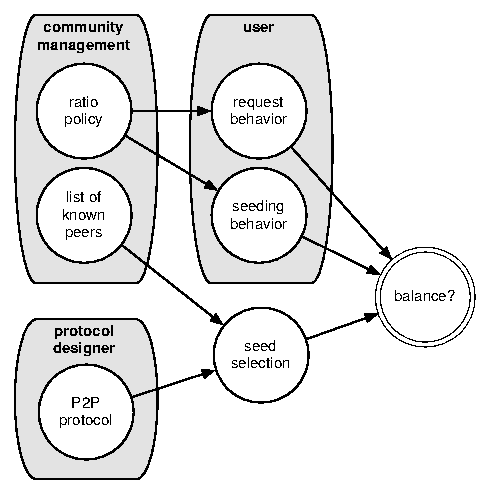
\includegraphics[width=0.7\textwidth]{pics/p2psys_balance.pdf}
	\caption{System properties and its relation to P2P balance \cite{2011:managesupplydemand:meulpolder}.}.
	\label{fig:sysbalance}
\end{figure}

% balance -> not sustain
\citeauthor{2011:managesupplydemand:meulpolder} in his work illustrated the relation between various P2P system properties and its relation to system balance. The illustration is shown in figure \ref{fig:sysbalance}. In his work, \citeauthor{2011:managesupplydemand:meulpolder} showed that by using naive random seeding behavior, it is not sufficient to make the P2P system  balanced \cite{2011:managesupplydemand:meulpolder}. An unbalance system can not only lead to an unsustainable community but also worsen the user download experience. Therefore, it is important to study seeding behavior for each peer to find out how to balance supply and demand in \bt~swarms.

\subsection{Investing as seeding behavior}
% Distinction invest vs donate.
The activity of spending credit can be divided into three categories: (i) \textit{trading}, (ii) \textit{investing}, and (iii) \textit{gifting} or \textit{donating}. When a user wants to spend their credit to get something, we define it as \textit{trading} or buying. \textit{Gifting} is the case in which a peer consciously intends to not get any direct, immediate, or obvious return for their spent credits \cite{2006:gifting:ripeanu}. The purpose of this action is usually to improve the performance of a community, or simply to demonstrate altruism. Investment is the activity of spending credit with the expectation of obtaining credit to use later on. 

%This is the most common case because in a credit-based community, every content has its price.

% helping others in p2p, improve performance
%Recent work on helping other user to increase downloading performance using \bt~ has been done. \citeauthor{2014:cloudseed:leon} uses \bt~ protocol to increase user download speed and at the same time reduce datacenters load. They analyze which swarm or file to help using user bandwidth information and number of connected user\cite{2014:cloudseed:leon}. From another perspective, \citeauthor{2015:coalitionbt:zhang} introduced the \textit{coalition} between \bt~ peers. Coalition is a set of peers that cooperate each other in regards to \bt~policy to minimize download completion time. They also propose coalition-compatible choking strategy to replace the current \bt~one. This research lead to significant performance improvement within the coalition \cite{2015:coalitionbt:zhang}. Although not using \bt~protocol, in \citeyear{2009:p2phelp:he}, \citeauthor{2009:p2phelp:he} proved that helper peer also can improve the streaming capacity in P2P system\cite{2009:p2phelp:he}. \citeauthor{2016:gameauctionp2pstream:mostafavi} extend this work by introducing auction aspect for uploader to choose which user will receive the bandwidth he donate \cite{2016:gameauctionp2pstream:mostafavi}. \citeauthor{2016:gameauctionp2pstream:mostafavi} used game-theory to propose new framework in uncooperative peers with maximizing the credit gain for helpers.

% the importance of healthy swarm -> public good, prevent tragedy of the common. user is selfish, it is good to donate. Reality : they want something in return -> credit. Move the problem into investment problem. 
The ideal situation to balance the performance and sustainability in \bt~communities is obtained by aligning supply and demand as discussed in section \ref{section:suppdemand}. Aside from \textit{trading} which is a natural occurrence in \bt~communities, by \textit{gifting} undersupplied swarms adequately, the optimal situation can be achieved, and the tragedy of the common can be prevented \cite{2002:reputationtotragedy:milinski}. However, P2P users are typically selfish in an economic perspective \cite{2014:userbehaviourprivate:jia}. \citeauthor{2009:demandsupplyres:andrade} also shows that users who contribute more to the community, actually consume more from it than lesser contributors \cite{2009:demandsupplyres:andrade}. This explains why \bt~users are not sufficiently altruistic. Therefore, \textit{investment} as a seeding behavior is the most feasible method to balance user and community needs.

We define the activity of downloading with the expectation of obtaining credit in the future (by uploading) as \textit{investment}. A user can \textit{prospect} which swarm he will invest in irrespective of his resource. The process of identifying the swarm that needs to be seeded is important to balance content availability and personal gain. In a good investing algorithm, users can gain credits and help each other. By providing proper prospecting function, the investment can be more accurate.

%By providing proper prospecting function, users could help each other to improve a swarm quality. In a good investing algorithm, users can make better use of its resource to gain credits.

% find low price, sell high price
In classical economic principle, the key to gain benefit is to buy low and sell high. By finding popular items and suitable swarms, the potential of investment become huge. For example, in the case of flashcrowd, an item can become so popular that undersupply might happen. The flashcrowd effect is the sudden increase in demand due to various reasons. For instance, a recently published torrent is one of the cases in which the flashcrowd effect takes place \cite{2013:swarmevolution:su}. Investing in the flashcrowd swarms is more beneficial compared to the old, saturated swarms. Furthermore, supply and demand misalignments can be avoided.

%If all users can download from oversupplied swarm and also upload to undersupplied swarm, it will reduce the misalignments on those two cases. Specifically, uploading to undersupplied swarm will increase the probability of gaining high credit.

% However, this property depends on the item and the market condition. If we translate it into \bt~ economic environment, the item is the file, and the condition is the swarm. \citeauthor{2012:economicbt:kash} introduced term is \textit{resale value}. Resale value is the amount of \textit{gross} credit one will get by uploading a file. In DIME case, it is 4 times uploaded bytes. In other words, resale value is the amount of return one can expect by uploading a file. We saw this mechanism as a way to incentivize user. Because by uploading one byte, a user can get 4 credit which can be used to spend/download 4 bytes. 




%\\
%Anonymous Relaying performance in Tribler \cite{2015:onionroutetribler:stokkink}\\
%Significant portion when seeding million torrents \cite{2012:milliontorrent:arvid}
%
%check swarm scrape -> multiple research -> based on dump logs

% piece population study -> http://ieeexplore.ieee.org/document/4410992/?arnumber=4410992
% related : Legout's work

% characteristics : http://www.sciencedirect.com/science/article/pii/S1389128610003622

\section{Prior Credit Mining Research}
\label{section:cmprior}
Our work is based on the preliminary work by \citeauthor{2015:creditmining:capota} from 2013 till 2015 \cite{2015:creditmining:capota, 2013:investmentcm:capota, 2014:bwmarket:capota}. Based on the prototype they made, a complex method with a speculative download to assess the swarms was implemented \cite{2013:investmentcm:capota}. Extending this work, they introduced a \textit{helper} peer to seed low capacity swarms using libtorrent \textit{share mode} \cite{2014:bwmarket:capota}. Recently, they moved to a multiple swarm approach and used a public community as their research object. With swarm selection policy, they observed whether helper peers could generate high credit with less downloading \cite{2015:creditmining:capota}. \citeauthor{2015:creditmining:capota} conducted emulation and simulation in their work.

\begin{figure}[h]
	\centering
	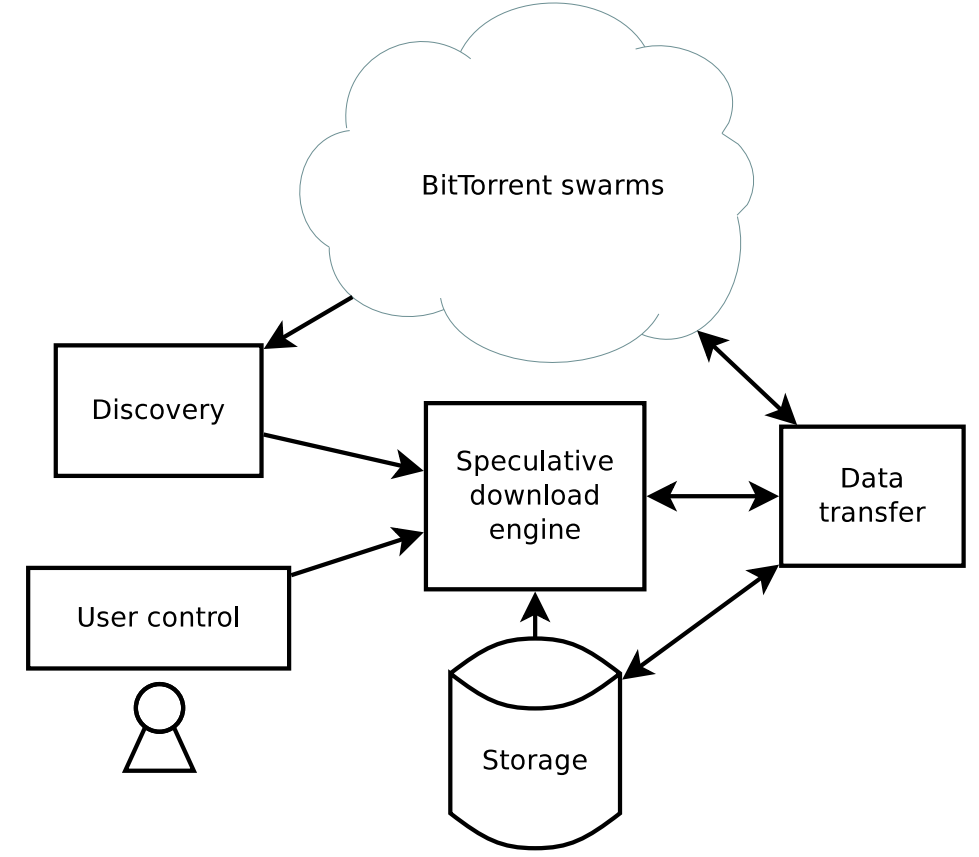
\includegraphics[width=0.7\textwidth]{pics/SDE2013.png}
	\caption{Speculative download mechanism \cite{2013:investmentcm:capota}}.
	\label{fig:sde13}
\end{figure}

In \citeyear{2013:investmentcm:capota}, \citeauthor{2013:investmentcm:capota} introduced bandwidth investing in \bt~private communities. They applied speculative download (as shown in figure \ref{fig:sde13}) on a prospective swarm. This research used activity data crawled from Bitsoup\footnote{\url{https://www.bitsoup.me}} to evaluate their system. Every swarm is analyzed as to whether the system keeps the swarm in \textit{cache} or discards it. The swarm is scored by predicting future upload speeds defined in the multiple regression model \cite{2013:investmentcm:capota}. One of the limitations is that the more swarms that need to be assessed, the less chance there is that the algorithm will find a suitable cache to replace. Another limitation is that \textit{multivariate adaptive regression splines} (MARS) implemented in this system is very costly and complex.

A year later, in \citeyear{2014:bwmarket:capota},  research to align supply and demand in \bt~network was conducted. Each peer monitored their swarms to detect potential undersupply. If such a condition is found, a peer broadcasted a \textit{help request} to specialized peers in order to seed that particular swarm. Specialized peers, called \textit{helpers}, try to download as little as possible while uploading as much as possible using \textit{libtorrent} share mode. They implement multiple helpers and observe its effect on the swarm. The result of their experiment shows that using share mode in a closed environment increases download performance  by shifting the bottleneck in the swarm if the bandwidth is underutilized \cite{2014:bwmarket:capota}. 

The most recent work was conducted in \citeyear{2015:creditmining:capota} \cite{2015:creditmining:capota}. \citeauthor{2015:creditmining:capota} incorporated their previous work into a Credit Mining System. The credit mining system is able to monitor multiple swarms in one moment, and can then decide to which swarm this system will give its bandwidth. It uses a simpler policy to choose a swarm compared to the multivariate regression model in previous work \cite{2013:investmentcm:capota}. The overview of the mining process is shown in figure \ref{fig:cm15}. The experiment was conducted in a live fashion on the \textit{etree.org}\footnote{\url{http://bt.etree.org/rss/bt\_etree\_org.rdf}} public community. They observed a \textit{net upload gain} which is defined as a positive difference in uploaded bytes and downloaded bytes. The proposed policy and framework resulted in positive effects to both the community and individuals.

\begin{figure}[ht]
	\centering
	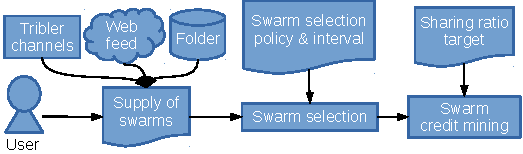
\includegraphics[width=0.8\textwidth]{pics/creditmining2015.pdf}
	\caption{The overview of credit mining process \cite{2015:creditmining:capota}}.
	\label{fig:cm15}
\end{figure}


\section{Prospecting good investment}

% emphasize on investing+prospect
Investing cannot be separated from another activity known as ``prospecting''. We define \textit{prospecting} as the activity of identifying and measuring a swarm in the hope of getting good \textit{return-of-investment}. In practice, not all undersupplied swarms need to be seeded, even more oversupplied swarms. A swarm can be chosen by considering its seeder-to-leecher ratio, piece availability, resource availability, and many more factors. In a credit based community, on point investment may spark the community thus improving the performance. From the user perspective, a good prospecting algorithm can result in an increased possibility of high return-of-investment.

% crawl -> part of prospecting, knowing the swarm. 
Getting swarm information is crucial for prospecting. Most researchers have measured \bt~ swarm by crawling its respective community pages \cite{2013:survivepriv:jia, 2005:bittorrentcooperation:andrade, 2014:userbehaviourprivate:jia, 2010:pubpriv:meulpolder, 2014:sustainabilitytorrent:chen, 2012:economicbt:kash, 2013:investmentcm:capota, 2009:demandsupplyres:andrade, 2011:interswarm:capota}. This way, the researchers can get the data summarized by the pages. Some researchers contact the tracker regularly or use its dump logs \cite{2011:yoshida:crawlbtnet, 2005:bittorrentcooperation:andrade,  2015:freeriderinbtcommunity:das, 2011:interswarm:capota}. Most of the research that has used logs as its dataset only used a single tracker to monitor a particular torrent. BTWorld\footnote{\url{http://btworld.nl/}} has identified four measurement techniques in \bt~\cite{2010:btworld:wojciechowski} as shown in table \ref{tbl:btmeasuremethod}. As investment needs real-time data, both \textit{swarm-level} and \textit{peer-level} measurement seems to be the most compatible with prospecting method implementation. Both \textit{internet-level} and \textit{community-level} needs compiled data from the ISP company and community administrators, respectively.

%Few of the research use instrumented client or directly observe the \bt~environment by understanding peer behavior \cite{2010:pubpriv:meulpolder, 2013:swarmevolution:su}.  

\begin{table}[ht]
	\centering
	\caption{\bt~measurement techniques \cite{2010:btworld:wojciechowski}.}
	\label{tbl:btmeasuremethod}
	\begin{tabular}{|l|l|l|l|}
		\hline
		\rowcolor[HTML]{C0C0C0} 
		\multicolumn{1}{|c|}{\cellcolor[HTML]{C0C0C0}\textbf{Level}} & \multicolumn{1}{c|}{\cellcolor[HTML]{C0C0C0}\textbf{Advantage}} & \multicolumn{1}{c|}{\cellcolor[HTML]{C0C0C0}\textbf{Disadvantage}} & 
		\multicolumn{1}{c|}{\cellcolor[HTML]{C0C0C0}\textbf{Source}}\\ \hline
		Internet & Excellent coverage & ISP collaboration & P2P traffic \\ \hline
		Community & Implementation & Peer details & Tracker logs \\ \hline
		Swarm & Details & Context & Tracker scraping \\ \hline
		Peer & Details & Scalability & Peers communication \\ \hline
	\end{tabular}
\end{table}

\subsection{Credit mining as investment tool}

The idea of the credit mining system is to help under-capacity swarms, while at the same time getting credit for uploading data. The system needs to find swarms that might have high return in \textit{prospecting}. The \textit{investing}, which relies on prospecting, is more complex. It has to consider used, limited resources as an additional requirement. The resource can be in several forms, such as bandwidth, memory, or storage. Although the term ``good'' may be relative, we wish to demonstrate the performance of the system by measuring how much net credit it gained. Therefore, we define the first research question as:

\noindent{
	\\
	\textit{How to prospect swarms and what is a good investment?}\\
	}
	
%How do we take advantage of unused bandwidth in Tribler client in non-disruptive manner?  The system address this issue by proposing activity-aware mechanism. The purpose is to get the most out of the bandwidth without disturb user of his own activity.
% What is the effect of credit mining system in live production environment?
In order to answer the question, we formulate technical challenges that need to be solved. The challenges include the engineering and performance evaluation aspect. Both prospecting and seeding processes may disrupt user activity. Therefore, it is important to take advantage of any unused bandwidth. Many characteristics of a swarm, such as seeder ratio and swarm completeness, need to be considered. The system will need to quantify those characteristics into a value which can be compared and evaluated. The goal is to build an autonomous prospecting and investing system that can yield a high return on investment. In evaluating the system, it is necessary to observe the effect of the credit mining system as a whole.

\section{Substituting investment cache}
In the first question, we have addressed how to gain as much credit as possible in a non-disruptive manner. However, this does not consider the limited resources available at the user's disposal. Investment is a tedious activity if it is done manually. Users are often forced to seed for an excessively long time to maintain adequate credit \cite{2013:survivepriv:jia}. By seeding unproductively, the user wastes their effort and resources, such as bandwidth and storage capacity. 

%In this issue, we will specifically focus on the storage limitation. The term \textit{storage} and \textit{cache} can be used interchangeably. It points to the container used to store the swarm data as the source of investment.

Before seeding can be started, the data must be available locally in the \textit{cache}. By having many data, there is a higher chance to seed multiple swarms as well. Eventually, it is necessary to replace obsolete investment. There are several reasons to do so such as gaining less profit, unstable credit, or unreliable swarms. By replacing an old swarm with a new swarm, the credit gained must remain stable or higher than before. Monitoring multiple swarms manually is unproductive. For that reason, it is desirable for us to do this automatically. Therefore, we define the second research question as: 

\noindent{
	\\
	\textit{When to delete a downloaded swarm and replace it with a new investment?}\\
	}
	
%What is the effect of mining in background for end-user?
The technical challenge that arises from this question covers several aspects. The characteristics of an unproductive swarm need to be defined. With regard to the previous question, it needs to be numerically comparable with another swarm. Because replacing a swarm is costly, there must be a precaution in place to help an unproductive swarm to yield more credits. In other words, a preventive mechanism needs to be formulated. If all the methods fail, a swarm that potentially gains higher credit needs to be chosen to replace the obsolete one. 